% subseccion 4.2
\subsection{Etapa 2: Búsqueda de Estudios}
\mbox{}\\
Esta etapa presenta la estrategia de búsqueda usada en la revisión sistemática de la literatura. Esta estrategia se describe en detalle en las subsecciones~\ref{subsubsec:Definiendo la Estrategia de Busqueda} -- \ref{subsubsec:resultados-busqueda}. Ver figura~\ref{fig:etapa2}.
\begin{figure*}[tbp]
    \centering
    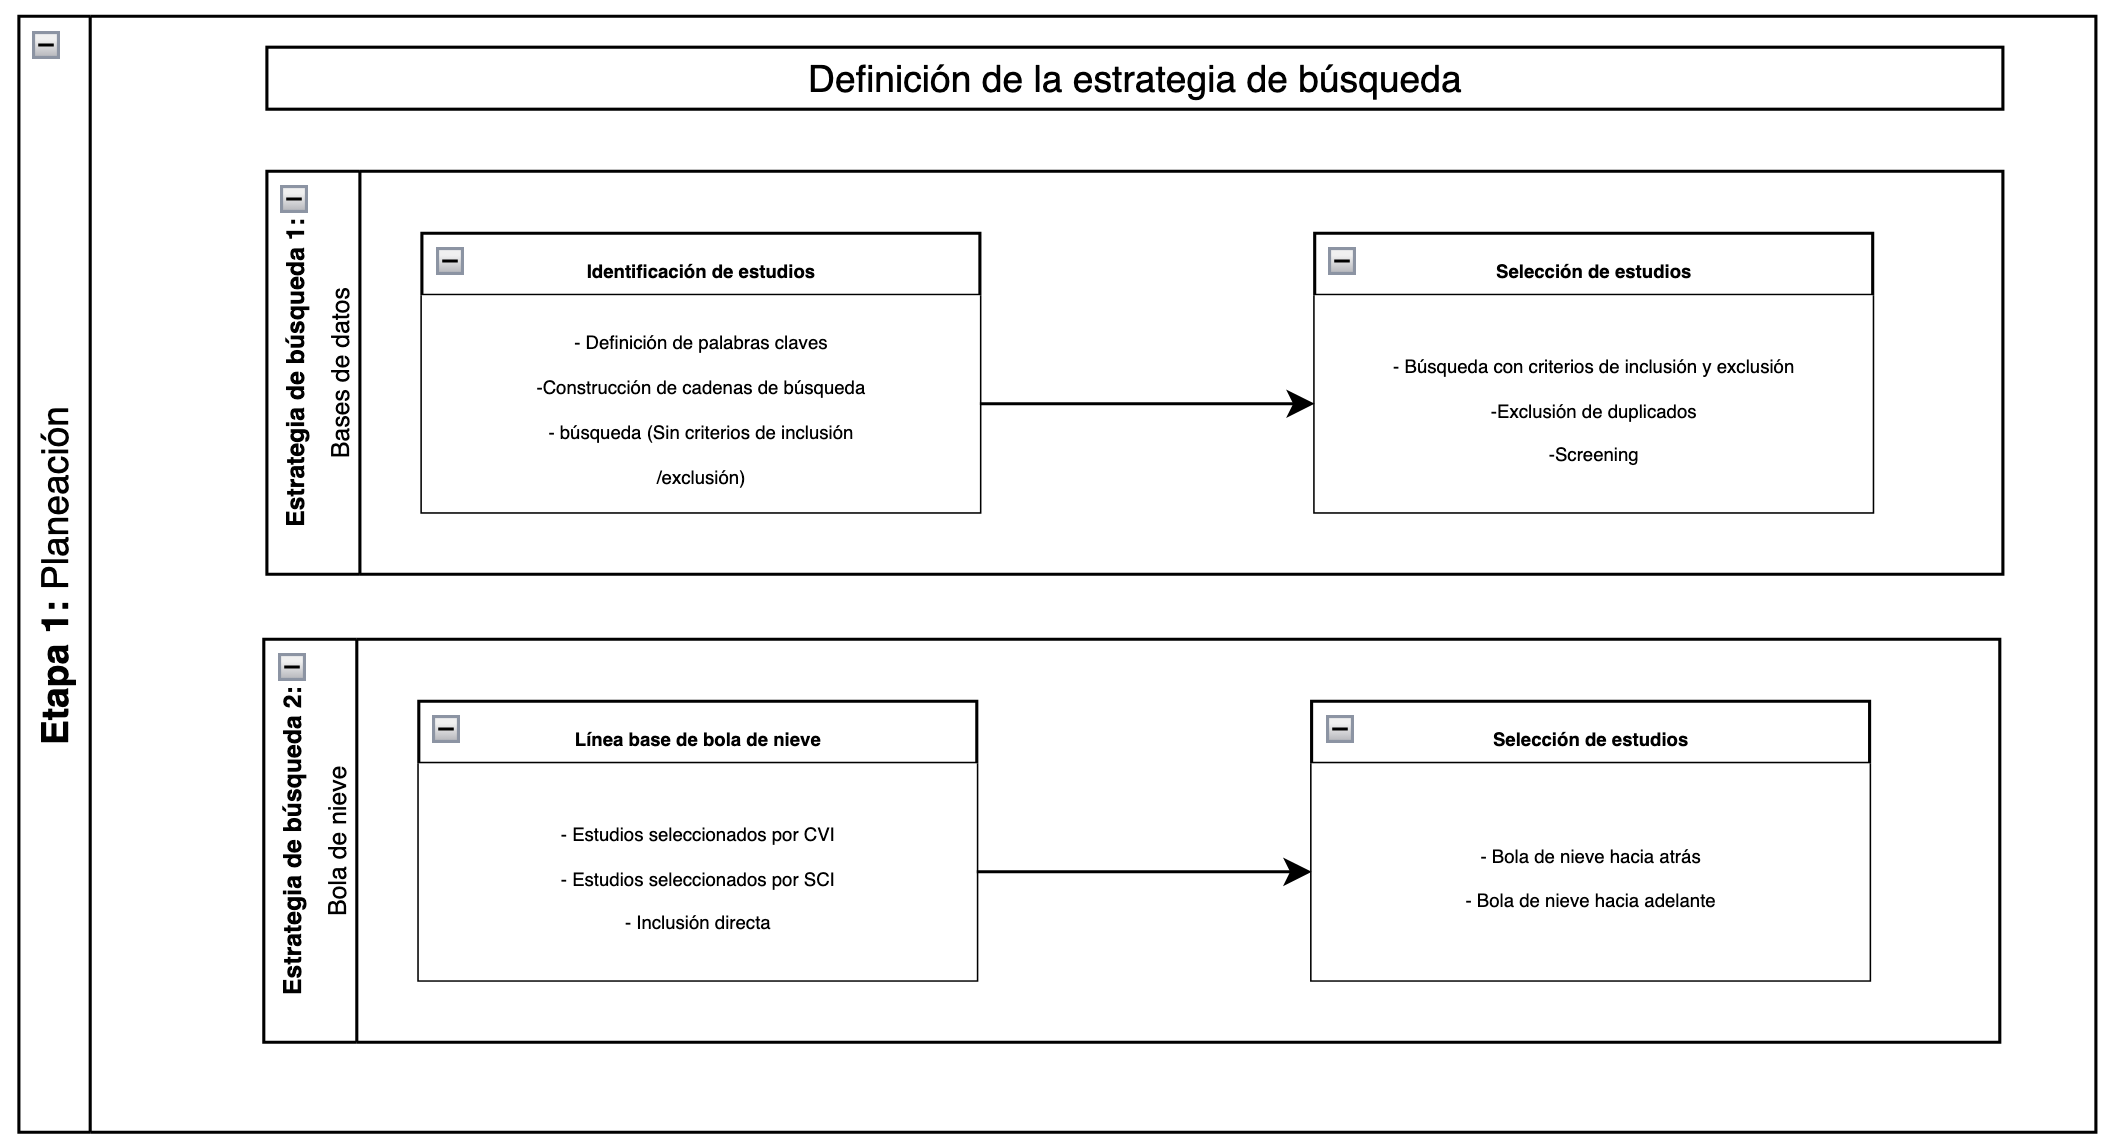
\includegraphics[width=0.9\textwidth,height=0.3\textheight]{resources/images/planeacion/estrategias-busqueda.png}
    \caption{Composición de la etapa de búsqueda de estudios}\label{fig:etapa2}
\end{figure*}
\mbox{}\\

%sub-subseccion 4.2.1 
\subsubsection{Definiendo la Estrategia de Búsqueda}\label{subsubsec:Definiendo la Estrategia de Busqueda}
\mbox{}\\
% Content for 4.2.1
Para la construcción de esta revisión de la literatura, se empleó un enfoque híbrido, cuyo propósito es ampliar el volumen de artículos indexados y diversificar sus orígenes, más allá de los proporcionados por las bases de datos.
En este sentido, se combinaron dos estrategias de búsqueda. La primera corresponde a la búsqueda en bases de datos, la cual consiste en ejecutar una cadena de búsqueda automatizada en repositorios académicos~\cite{jalali2012systematic}.
La segunda estrategia, denominada \textit{Snowballing} o ``bola de Nieve'', consiste en la búsqueda manual de artículos a partir de un conjunto base, utilizando tanto sus referencias como las citas que los mencionan. Esta estrategia parte de la premisa de que los estudios relevantes citan otros igualmente relevantes y, por lo tanto, permite encontrar trabajos que no están indexados en las bases de datos académicas~\cite{jalali2012systematic} y \cite{goodman1961snowball}.
\mbox{}\\
%sub-subseccion 4.2.2

\subsubsection{Estrategia de Búsqueda 1: Bases de Datos}
\mbox{}\\
Esta estrategia se divide en dos componentes. El primero, denominado ``Identificación de estudios'', se centra en definir las palabras clave para construir las cadenas de búsqueda que conducen a completar las búsquedas en las bases de datos académicas.
El segundo componente es llamado ``Selección de estudios'', se enfoca en aplicar diversos criterios para refinar la búsqueda de resultados de estudios y así maximizar el valor del SMS.

\begin{itemize}
    \item \textbf{Identificación de estudios: } Con el fin de favorecer la viabilidad del estudio y por acuerdo de los autores, se limitó la búsqueda a cinco bases de datos académicas: \textit{ACM}, \textit{IEEE Xplore}, \textit{Springer}, \textit{Science Direct} y \textit{Taylor and Francis}. En esta etapa del proceso fue necesario establecer las palabras claves definidas antes y construir cadenas de búsqueda específica para cada base de datos. Para ello,se empleó nuevamente el modelo PICOC como guía metodológica para identificar términos claves o frases completas que se relacionaban con \textbf{VBC}. En la construcción de dichas cadenas se incorporaron sinónimos con el próposito de ampliar el espectro de resultados. Ver cuadro~\ref{tab:palabras-clave}.\\
    Las principales palabras clave identificadas fueron: \textit{Container-based virtualization}, \textit{Education}, \textit{Research}, \textit{Industry}. Para ampliar y refinar los resultados se utilizaron operadores booleanos como \textit{AND} y \textit{OR}. Además, se emplearon comillas para la búsqueda de frases exactas y paréntesis para agrupar términos relacionados. El conjunto de palabras clave seleccionadas para construir las cadenas de búsqueda se presenta en el cuadro~\ref{tab:keywords}.\\
    Para dirigir la búsqueda hacia la intersección de los dominios de TI y la \textbf{VBC} se aplicó el operador booleano \textit{AND}. Una vez identificadas las palabras clave, se procedió con la construcción de las cadenas de búsqueda para cada base de datos, mediante un proceso iterativo. Dicho proceso consistió en la aplicación de un enfoque heurístico sobre palabras clave, sinónimos y conceptos relacionados, haciendo uso de conjunciones y disyunciones de acuerdo con las reglas específicas de cada base de datos. En consecuencia, las cadenas de búsqueda presentan variaciones según los criterios de cada repositorio. Ver cuadro~\ref{tab:cadenas-busqueda}.\\

    Una vez construidas las cadenas de búsqueda, estas se ejecutaron en cada base de datos. El cuadro~\ref{tab:resultados-busqueda-sin-criterio} presenta el conjunto de resultados obtenidos. En total, se identificaron \textbf{6530} preliminares, destacando que la base de datos \textit{Springer} es la que más resultados aportó, con un total de \textbf{4562} artículos, equivalente al \textbf{69.8\%} del total.

    \item \textbf{Selección de estudios: } Con el fin de refinar los resultados obtenidos, se aplicaron los criterios de inclusión y exclusión establecidos en la etapa de planeación. La tabla~\ref{tab:resultados-busqueda-criterios} muestra el resultado de este paso. Como resultado, el número de artículos se redujo a \textbf{976}. Entre ellos, Springer continuó siendo la base de datos con mayor aporte, con \textbf{592} artículos (\textbf{60.65\%} del total). Posteriormente, se identificaron y se eliminaron \textbf{274} artículos duplicados, obteniendo un total de \textbf{771} artículos únicos. Sobre este nuevo conjunto se aplicó un proceso de \textit{Screening} que consistió en la revisión del título, resumen y las palabras clave de cada artículo, con el fin de verificar su pertinencia y alineación con los objetivos del estudio.
    Este análisis permitió descartar \textbf{593} artículos por no aportar valor a la investigación, lo que resulta en un total de \textbf{110} estudios seleccionados. Con este paso concluye la estrategia de búsqueda en bases de datos. La figura \ref{fig:resumen-busqueda-bds} resume la metodología aplicada en este proceso.\\
\end{itemize}

\begin{table}[tbp]
    \scriptsize % reduce tamaño del texto
    \centering
    \renewcommand{\arraystretch}{1.3}
    \begin{tabularx}{\columnwidth}{>{\centering\arraybackslash}m{0.18\columnwidth} >{\RaggedRight\arraybackslash}X}
        \hline
        \textbf{Aspecto} & \textbf{Descripción} \\
        \hline
        Población & VBC, Dominios de TI, Educación, Investigación, Extensión \\
        Intervención & Identificación, Clasificación \\
        Comparación & Tasa de éxito, Evidencia de uso \\
        Salida & Clasificación de trabajos relacionados con VBC en cada dominio de TI \\
        Contexto & Docencia, Investigación, Extensión \\
        \hline
    \end{tabularx}
    \caption{Palabras clave identificadas usando el modelo PICOC}\label{tab:palabras-clave}
\end{table}

\begin{table}[tbp]
    \scriptsize % reduce tamaño del texto
    \centering
    \renewcommand{\arraystretch}{1.3}
    \begin{tabularx}{\columnwidth}{>{\centering\arraybackslash}m{0.18\columnwidth} >{\RaggedRight\arraybackslash}X}
        \hline
        \textbf{Palabras clave} & \textbf{Sinónimos} \\
        \hline
        Container-based virtualization & Application virtualization, Docker, Lightweight Virtualization \\
        Education & Education System, Education Development, Higher Education \\
        Research & Research Group, Research Proposal \\
        Industry & IT Services, Technology Infrastructure, Cloud Computing \\
        \hline
    \end{tabularx}
    \caption{Palabras clave para la búsqueda en base de datos}\label{tab:keywords}
\end{table}

\begin{table*}[tbp]
    \scriptsize % reduce tamaño del texto
    \centering
    \renewcommand{\arraystretch}{1.3}
    \begin{tabularx}{\textwidth}{>{\raggedright\arraybackslash}X 
                                 >{\centering\arraybackslash}X 
                                 >{\centering\arraybackslash}X 
                                 >{\centering\arraybackslash}X 
                                 >{\centering\arraybackslash}X 
                                 >{\centering\arraybackslash}X}
        \hline
        \textbf{Criterio} & \textbf{ACM} & \textbf{IEEE} & \textbf{Science Direct} & \textbf{Springer} & \textbf{Taylor and Francis} \\
        \hline
        Resultados de cadenas de búsqueda solo con palabras clave & 189 & 426 & 4562 & 353 & 1000 \\
        Porcentaje de contribución & 2.89\% & 6.52\% & 69.86\% & 5.4\% & 15.31\% \\
        \hline
    \end{tabularx}
    \caption{Resultados de búsqueda por base de datos usando palabras clave}\label{tab:resultados-busqueda-sin-criterio}
\end{table*}

\begin{table*}[tbp]
    \scriptsize % reduce tamaño del texto
    \centering
    \renewcommand{\arraystretch}{1.3}
    \begin{tabularx}{\textwidth}{>{\raggedright\arraybackslash}X 
                                 >{\centering\arraybackslash}X 
                                 >{\centering\arraybackslash}X 
                                 >{\centering\arraybackslash}X 
                                 >{\centering\arraybackslash}X 
                                 >{\centering\arraybackslash}X}
        \hline
        \textbf{Criterio} & \textbf{ACM} & \textbf{IEEE} & \textbf{Science Direct} & \textbf{Springer} & \textbf{Taylor and Francis} \\
        \hline
        Resultados de cadenas de búsqueda solo con palabras clave & 48 & 134 & 46 & 592 & 156\\
        Porcentaje de contribución & 4.91\% & 13.72\% & 4.71\% & 60.65\% & 15.98\%\\
        \hline
    \end{tabularx}
    \caption{Resultados de búsqueda por base de datos usando palabras clave}\label{tab:resultados-busqueda-criterios}
\end{table*}

\newcolumntype{P}[1]{>{\raggedright\arraybackslash}p{#1}}

\begin{table*}[htbp]
\centering
\scriptsize
\renewcommand{\arraystretch}{1.5}
\begin{adjustbox}{max width=\textwidth}
\begin{tabular}{|P{0.15\linewidth}|P{0.25\linewidth}|P{0.25\linewidth}|P{0.25\linewidth}|}
\hline
\textbf{Base de Datos / Dominio} & \textbf{Educación AND VBC} & \textbf{Investigación AND VBC} & \textbf{Industria AND VBC} \\
\hline

\textbf{ACM Digital Library} 
& \tiny \texttt{(Title:(``Container-based virtualization'' OR ``Application virtualization'' OR ``Docker'' OR ``Lightweight Virtualization'') AND Title:(``Education'' OR ``Education System'' OR ``Education Development'' OR ``Higher Education'')) OR (Abstract:(``Container-based virtualization'' OR ``Application virtualization'' OR ``Docker'' OR ``Lightweight Virtualization'') AND Abstract:(``Education'' OR ``Education System'' OR ``Education Development'' OR ``Higher Education'')) OR (Keyword:(``Container-based virtualization'' OR ``Application virtualization'' OR ``Docker'' OR ``Lightweight Virtualization'') AND Keyword:(``Education'' OR ``Education System'' OR ``Education Development'' OR ``Higher Education''))} 
& \tiny \texttt{(Title:(``Container-based virtualization'' OR ``Application virtualization'' OR ``Docker'' OR ``Lightweight Virtualization'') AND Title:(``Research'' OR ``Research Group'' OR ``Research Proposal'')) OR (Abstract:(``Container-based virtualization'' OR ``Application virtualization'' OR ``Docker'' OR ``Lightweight Virtualization'') AND Abstract:(``Research'' OR ``Research Group'' OR ``Research Proposal'')) OR (Keyword:(``Container-based virtualization'' OR ``Application virtualization'' OR ``Docker'' OR ``Lightweight Virtualization'') AND Keyword:(``Research'' OR ``Research Group'' OR ``Research Proposal''))} 
& \tiny \texttt{(Title:(``Container-based virtualization'' OR ``Application virtualization'' OR ``Docker'' OR ``Lightweight Virtualization'') AND Title:(``Industry'' OR ``IT Services'' OR ``Technology Infrastructure'' OR ``Cloud Computing'')) OR (Abstract:(``Container-based virtualization'' OR ``Application virtualization'' OR ``Docker'' OR ``Lightweight Virtualization'') AND Abstract:(``Industry'' OR ``IT Services'' OR ``Technology Infrastructure'' OR ``Cloud Computing'')) OR (Keyword:(``Container-based virtualization'' OR ``Application virtualization'' OR ``Docker'' OR ``Lightweight Virtualization'') AND Keyword:(``Industry'' OR ``IT Services'' OR ``Technology Infrastructure'' OR ``Cloud Computing''))} \\
\hline

\textbf{IEEE Xplore} 
& \tiny \texttt{((``Abstract'': ``Container-based virtualization'' OR ``Abstract'': ``Application virtualization'' OR ``Abstract'': ``Docker'' OR ``Abstract'': ``Lightweight Virtualization'') AND (``Abstract'': ``Education'' OR ``Abstract'': ``Education System'' OR ``Abstract'': ``Education Development''  OR ``Abstract'': ``Higher Education'')) OR ((``Publication Title'': ``Container-based virtualization'' OR ``Publication Title'': ``Application virtualization'' OR ``Publication Title'': ``Docker'' OR ``Publication Title'': ``Lightweight Virtualization'') AND (``Publication Title'': ``Education'' OR ``Publication Title'': ``Education System'' OR ``Publication Title'': ``Education Development''  OR ``Publication Title'': ``Higher Education'')) OR ((``Author Keywords'': ``Container-based virtualization'' OR ``Author Keywords'': ``Application virtualization'' OR ``Author Keywords'': ``Docker'' OR ``Author Keywords'': ``Lightweight Virtualization'') AND (``Author Keywords'': ``Education'' OR ``Author Keywords'': ``Education System'' OR ``Author Keywords'': ``Education Development''  OR ``Author Keywords'': ``Higher Education''))} 
& \tiny \texttt{((``Abstract'': ``Container-based virtualization'' OR ``Abstract'': ``Application virtualization'' OR ``Abstract'': ``Docker'' OR ``Abstract'': ``Lightweight Virtualization'') AND (``Abstract'': ``Research Group'' OR ``Abstract'': ``Research Proposal'')) OR ((``Publication Title'': ``Container-based virtualization'' OR ``Publication Title'': ``Application virtualization'' OR ``Publication Title'': ``Docker'' OR ``Publication Title'': ``Lightweight Virtualization'') AND (``Publication Title'': ``Research Group'' OR ``Publication Title'': ``Research Proposal'')) OR ((``Author Keywords'': ``Container-based virtualization'' OR ``Author Keywords'': ``Application virtualization'' OR ``Author Keywords'': ``Docker'' OR ``Author Keywords'': ``Lightweight Virtualization'') AND (``Author Keywords'': ``Research Group'' OR ``Author Keywords'': ``Research Proposal''))} 
& \tiny \texttt{((``Abstract'': ``Container-based virtualization'' OR ``Abstract'': ``Application virtualization'' OR ``Abstract'': ``Docker'' OR ``Abstract'': ``Lightweight Virtualization'') AND (``Abstract'': ``Industry'' OR ``Abstract'': ``IT Services'' OR ``Abstract'': ``Technology Infrastructure'' OR ``Abstract'': ``Cloud Computing'')) OR ((``Publication Title'': ``Container-based virtualization'' OR ``Publication Title'': ``Application virtualization'' OR ``Publication Title'': ``Docker'' OR ``Publication Title'': ``Lightweight Virtualization'') AND (``Publication Title'': ``Industry'' OR ``Publication Title'': ``IT Services'' OR ``Publication Title'': ``Technology Infrastructure'' OR ``Publication Title'': ``Cloud Computing'')) OR ((``Author Keywords'': ``Container-based virtualization'' OR ``Author Keywords'': ``Application virtualization'' OR ``Author Keywords'': ``Docker'' OR ``Author Keywords'': ``Lightweight Virtualization'') AND (``Author Keywords'': ``Industry'' OR ``Author Keywords'': ``IT Services'' OR ``Author Keywords'': ``Technology Infrastructure'' OR ``Author Keywords'': ``Cloud Computing''))} \\
\hline

\textbf{ScienceDirect} 
& \tiny \texttt{(``Container-based virtualization'' OR ``Application virtualization'' OR ``Docker'' OR ``Lightweight Virtualization'') AND (``Education'' OR ``Education System'' OR ``Education Development'' OR ``Higher Education'')} 
& \tiny \texttt{(``Container-based virtualization'' OR ``Application virtualization'' OR ``Docker'' OR ``Lightweight Virtualization'') AND (``Research'' OR ``Research Group'' OR ``Research Proposal'')} 
& \tiny \texttt{(``Container-based virtualization'' OR ``Application virtualization'' OR ``Docker'' OR ``Lightweight Virtualization'') AND (``Industry'' OR ``IT Services'' OR ``Technology Infrastructure'' OR ``Cloud Computing'')} \\
\hline

\textbf{SpringerLink} 
& \tiny \texttt{(title:(``Container-based virtualization'' OR ``Application virtualization'' OR ``Docker'' OR ``Lightweight Virtualization'') AND title:(``Education'' OR ``Education System'' OR ``Education Development'' OR ``Higher Education'')) OR (abstract:(``Container-based virtualization'' OR ``Application virtualization'' OR ``Docker'' OR ``Lightweight Virtualization'') AND abstract:(``Education'' OR ``Education System'' OR ``Education Development'' OR ``Higher Education'')) OR (keyword:(``Container-based virtualization'' OR ``Application virtualization'' OR ``Docker'' OR ``Lightweight Virtualization'') AND keyword:(``Education'' OR ``Education System'' OR ``Education Development'' OR ``Higher Education''))} 
& \tiny \texttt{(title:(``Container-based virtualization'' OR ``Application virtualization'' OR ``Docker'' OR ``Lightweight Virtualization'') AND title:(``Research'' OR ``Research Group'' OR ``Research Proposal'')) OR (abstract:(``Container-based virtualization'' OR ``Application virtualization'' OR ``Docker'' OR ``Lightweight Virtualization'') AND abstract:(``Research'' OR ``Research Group'' OR ``Research Proposal'')) OR (keyword:(``Container-based virtualization'' OR ``Application virtualization'' OR ``Docker'' OR ``Lightweight Virtualization'') AND keyword:(``Research'' OR ``Research Group'' OR ``Research Proposal''))} 
& \tiny \texttt{(title:(``Container-based virtualization'' OR ``Application virtualization'' OR ``Docker'' OR ``Lightweight Virtualization'') AND title:(``Industry'' OR ``IT Services'' OR ``Technology Infrastructure'' OR ``Cloud Computing'')) OR (abstract:(``Container-based virtualization'' OR ``Application virtualization'' OR ``Docker'' OR ``Lightweight Virtualization'') AND abstract:(``Industry'' OR ``IT Services'' OR ``Technology Infrastructure'' OR ``Cloud Computing'')) OR (keyword:(``Container-based virtualization'' OR ``Application virtualization'' OR ``Docker'' OR ``Lightweight Virtualization'') AND keyword:(``Industry'' OR ``IT Services'' OR ``Technology Infrastructure'' OR ``Cloud Computing''))} \\
\hline

\textbf{Taylor \& Francis} 
& \tiny \texttt{(``Application virtualization'' OR ``Docker'' OR ``Lightweight Virtualization'' OR ``Docker Container'') AND (``Education System'' OR ``Education Sector'' OR ``Education Development'' OR ``Higher Education'')} 
& \tiny \texttt{(``Application virtualization'' OR ``Docker'' OR ``Lightweight Virtualization'' OR ``Docker Container'') AND (``Specific Research Areas'' OR ``Research Group'' OR ``Research Proposal'' OR ``Research and Development'')} 
& \tiny \texttt{(``Application virtualization'' OR ``Docker'' OR ``Lightweight Virtualization'' OR ``Docker Container'') AND (``Industry'' OR ``IT Services'' OR ``Technology Infrastructure'' OR ``Cloud Computing'')} \\
\hline

\end{tabular}
\end{adjustbox}
\caption{Cadenas de búsqueda por base de datos y dominio}\label{tab:cadenas-busqueda-transpuesta}
\end{table*}


\begin{figure}[tbp]
    \centering
    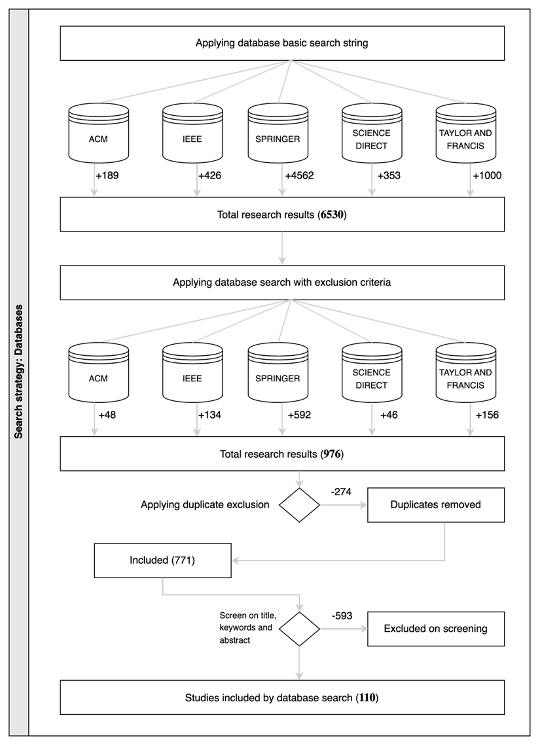
\includegraphics[width=0.5\textwidth]{resources/images/busqueda-estudios/busqueda-bd.png}
    \caption{Resumen de las actividades y resultados obtenidos en la estrategia de búsqueda en base de datos}\label{fig:resumen-busqueda-bds}
\end{figure}

% sub-subsetion for 4.2.3
\subsubsection{Estrategia de Búsqueda 2: Bola de Nieve}
\mbox{}\\
La estrategia de búsqueda de bola de nieve inició con la identificación del conjunto base de artículos. Este conjunto base se obtiene de la estrategia de búsqueda 1. Este procedimiento consistió en dos fases: en la primera, se revisaron las referencias de cada artículo para identificar nuevos trabajos (bola de nieve hacia atrás); en la segunda, se analizaron los artículos que citaban al conjunto base (bola de nieve hacia adelante), lo cual requirió el uso de bases de datos que proveen esta información. En ambas fases se aplicaron los criterios de inclusión y exclusión establecidos durante la etapa de planeación \cite{10.1145/2601248.2601268}. \\ \\
La primera fase, denominada \textit{Construcción de la línea base}, tiene como objetivo establecer los artículos sobre los cuales se realizarán un análisis de citas y referencias. Para conformar este conjunto inicial de estudios, se aplicaron diversos criterios, entre ellos el CVI \textit{(Content Value Index)}, el SCI \textit{(Study Citation Index)} y el criterio de inclusión directa. La segunda fase, denominada \textit{Selección de estudios}, se centra en el análisis de las referencias \textit{(Backward Snowballing)} y de las citas \textit{(Forward Snowballing)} correspondientes a cada artículo. \\ \\
La construcción de la línea base parte de los \textbf{110} artículos obtenidos en la estrategia de búsqueda en bases de datos. De este conjunto, se seleccionaron \textbf{25} artículos aplicando el critero de calidad SCI. La elección de este criterio se fundamenta en que no depende de la valoración de los autores, sino que se basa en la cantidad de citas recibidas por cada artículo, lo cual constituye un indicador objetivo de relevancia académica. El resultado de este proceso fue un total de \textbf{25} artículos seleccionados para la línea base. La selección se realizó mediante un análisis de frecuencia de citas, del cual se extrajo el primer cuartil \textbf{(Q1)} correspondiente a los artículos más citados.\\ \\
Como parte del proceso del SMS, es posible incorporar estudios mediante inclusión directa. Este procedimiento consiste en añadir al estudio un artículo previamente conocido por los autores, sin que provenga directamente de una base de datos. Este enfoque aporta flexibilidad al proceso de búsqueda ya que permite integrar trabajos que los autores consideran relevantes para el objetivo de la investigación. En este caso, se incorporó un artículo mediante inclusión directa, lo que llevó a un total de \textbf{26} artículos en la línea base.\\ \\
Tras la construcción de la línea base, se procedió con el análisis de las referencias, lo que permitió identificar un total de \textbf{495} artículos nuevos. El proceso de búsqueda hacia adelante fue realizado haciendo uso de Google Scholar, el cual proporciona información sobre el número de citas de cada artículo, siguiendo las practicas descritas en~\cite{8747000}. 
En cuanto a la búsqueda hacia atrás, se obtuvieron \textbf{87} artículos adicionales.\\

Se eliminaron \textbf{14} artículos duplicados entre los resultados de las búsquedas hacia atrás y hacia adelante. Posteriormente, se aplicó nuevamente el proceso de \textit{Screening}, que al igual que en la fase anterior, consistió en revisar el título, resumen y palabras clave de cada trabajo. Este procedimiento permitió reducir a \textbf{116} los artículos seleccionados mediante la estrategia de búsqueda por bola de nieve. La figura~\ref{fig:resumen-busqueda-snowballing} presenta un resumen del proceso seguido en esta estrategia de búsqueda.\\ \\
\mbox{}

\begin{figure}[tbp]
    \centering
    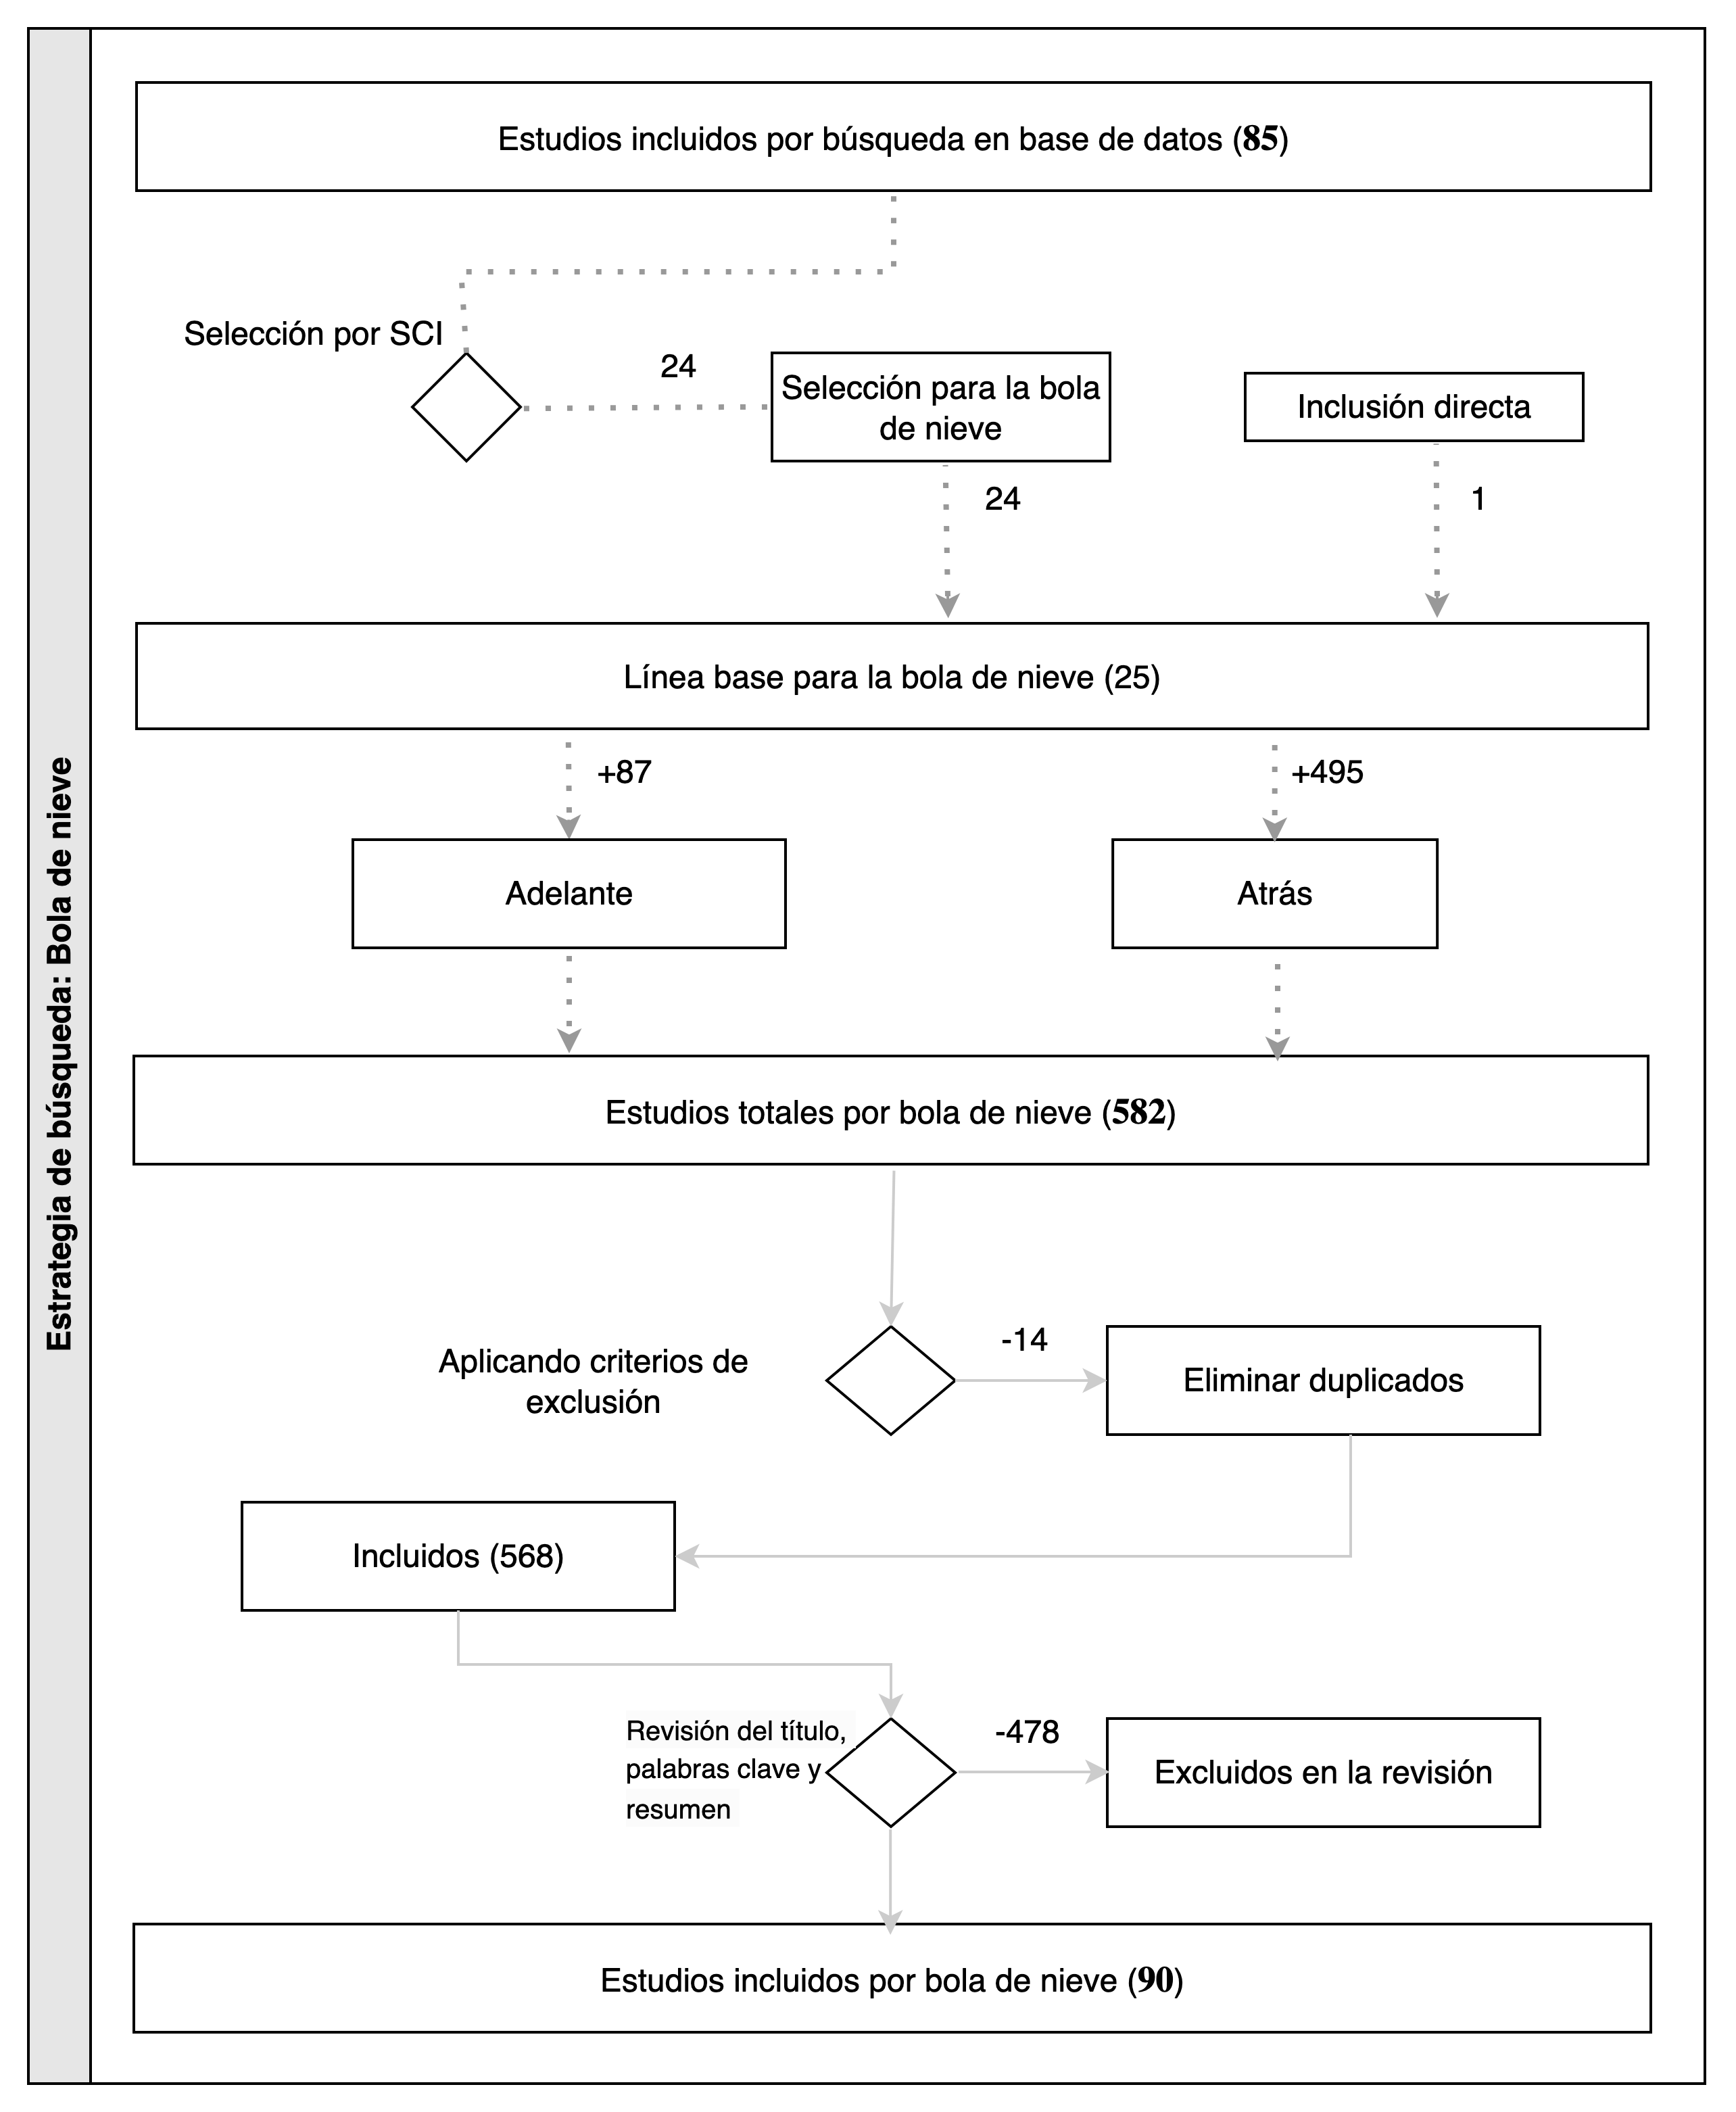
\includegraphics[width=0.5\textwidth]{resources/images/busqueda-estudios/busqueda-snowball.png}
    \caption{Resumen de la estrategia de búsqueda - Bola de nieve}\label{fig:resumen-busqueda-snowballing}
\end{figure}

\begin{table}[htbp]
\renewcommand{\arraystretch}{1.3}
\begin{tabularx}{\columnwidth}{
    >{\centering\arraybackslash}m{0.3\textwidth}
    >{\centering\arraybackslash}X
    >{\centering\arraybackslash}m{0.15\textwidth}
}
\toprule
\textbf{Estrategia} & \textbf{Estudios} & \textbf{\%} \\
\midrule
Bases de Datos & 110 & 48.67\% \\
Bola de Nieve & 115 & 50.88\% \\
Inclusión Directa & 1 & 0.44\% \\
\textbf{Total} & \textbf{226} & \textbf{100\%} \\
\bottomrule
\end{tabularx}
\caption{Resultados de la búsqueda de estudios}\label{tab:resultados-busqueda}
\end{table}

% sub=-subsection 4.2.4
\subsubsection{Resultados de la Búsqueda de Estudios}\label{subsubsec:resultados-busqueda}
\mbox{}\\
Finalmente, la búsqueda de artículos se resume en \textbf{110} estudios obtenidos a través de bases de datos académicas, \textbf{116} estudios identificados mediante bola de nieve y \textbf{1} por inclusión directa (el cual se contabiliza en la bola de nieve), para un total de \textbf{226} estudios identificados. El cuadro~\ref{tab:resultados-busqueda} presenta un resumen de estos resultados.
\mbox{}\\